\chapter{Riemann Pump Circuit design - Implementation of the Riemann Pump approach}
Based on the idea a digital to analog converter is designed. Hence it is for the transmitting path and also the energy consumption suggest that it would be in a base station. So the deisgned device should be integrated in a base station transmitter path.
Approach of the push-pull stage Maksimovic, Maroldt.\\
Approach of theoretical and synthesized signal -> MatLab generation of Riemanncode, SNR.\\ Stability, driver concept, energy consumption, frequency bandwidth, gain
Schematic design in Advanced Design System 2014. concept, ideas... 
\textbf{length of the bonds, number of bonds, thickness of bonds ask Dirk Meder. A lot of vias - more inductance - voltage drop between layers. short as possible lines, no rechtecke - para caps in the edge. first filter cap to supply pin near the chip. number and cap size determined on experience. }\\
Control voltage of 5 V realization with OPAMPS? Possible to overdrive opamps instead of using broadband ppa. 

\begin{figure}[ht]
	\centering
  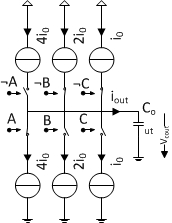
\includegraphics[width=0.4\textwidth]{RiemannPumpConcept.png}
	\caption{Concept of the Riemann Pump with Voltage Sources}
	\label{RiemannPumpConcept}
\end{figure}

The concept of the Riemann Pump as seen in Fig. \ref{RiemannPumpConcept} is realised with the design tool ADS.

\begin{figure}[ht]
	\centering
  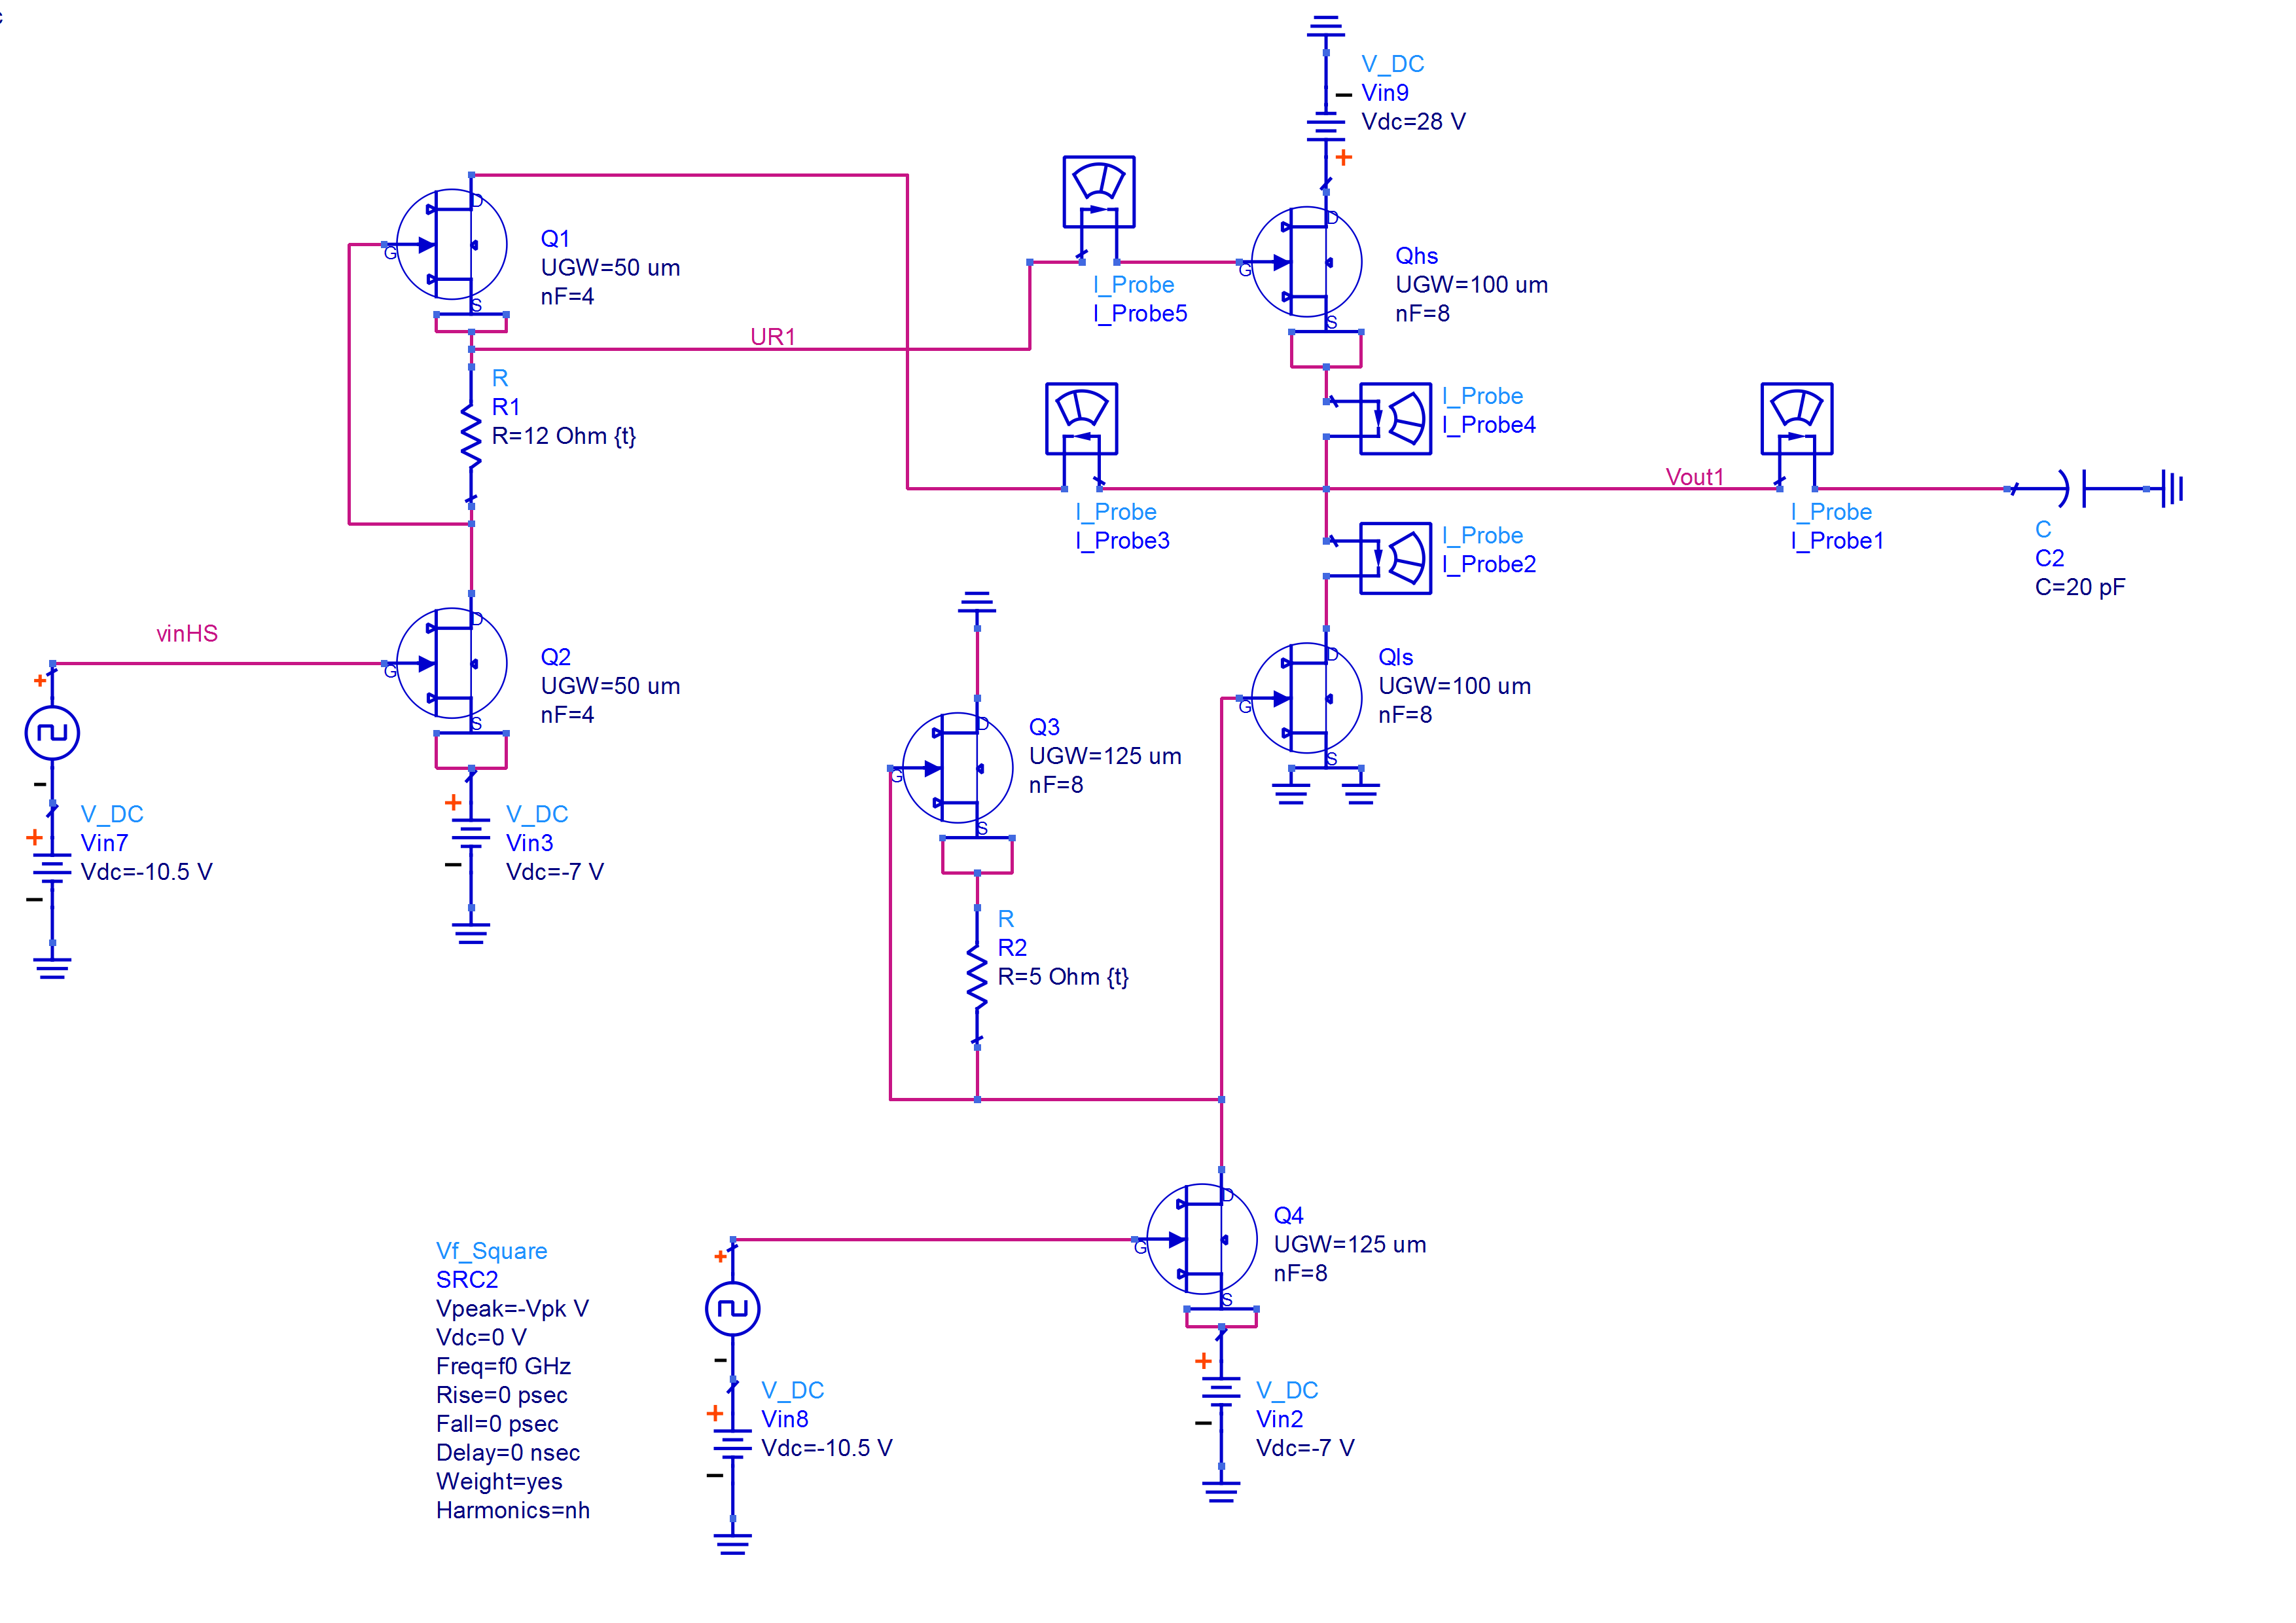
\includegraphics[width=1\textwidth]{Active_PullUp3.png}
	\caption{Schematic of the Riemann Pump circuit}
	\label{RiemannPumpConcept}
\end{figure}